\section{Applying Linux kernel}
\label{sec:linux}

%\subsection{Reverse mapping}

%$$$$$$$$$$$$$$$$$$$$$$$$$$$$$$$$$$$$$$$$$$$$$$$$$$$$$$$$$$$$$$$$$$$$$$$$$$$$$$$$
%Paragraph 1: Linux의 reverse mapping에 대한 자세한 설명 
%$$$$$$$$$$$$$$$$$$$$$$$$$$$$$$$$$$$$$$$$$$$$$$$$$$$$$$$$$$$$$$$$$$$$$$$$$$$$$$$$

This section shows how to apply the \LDU to the complex Linux
virtual memory system 
to solve the update serialization problem;it deals with more practical one.

The Linux reverse page mapping(rmap), a kernel memory management mechanism, consists
of anonymous rmap and file rmap, are a update-heavy data structure.
These two rmaps maintain virtual address(VMAs) to translate physical
addresses to virtual address~\cite{Dave2004OLSRMAP}, and the rmaps are a shared global resource between processes.
These global resource of rmap are managed by using a interval tree.
To protect these shared tree, Linux kernel uses the reader-writer semaphore, and simultaneous creation of many processes becomes bottlenecks because
not only the rmap's update operations can not run
in parallel but also update's lock brings about the cache invalidation traffic.
On the contrary, the rmap rarely reads the interval tree when it swaps a physical page
out to disk, migrates other cpu, or truncates a file.
%In brief, the Linux rmaps are a update-heavy data structure. 

\subsection{Anonymous mapping}

\begin{figure}[tb]
  \begin{center}
     \includegraphics[width=1\textwidth,height=1\textheight,keepaspectratio]{fig/anon_vma}
  \end{center}
  \caption{An example of applying the \LDU to anonymous reverse mapping.
  When a process simultaneously spawns, the root lock leads to a scalability bottleneck. 
  The log's queue is added into the per-core memory or the
  global head object(\code{struct anon\_vma})}
  \label{fig:anonvmaramp}
\end{figure}

%$$$$$$$$$$$$$$$$$$$$$$$$$$$$$$$$$$$$$$$$$$$$$$$$$$$$$$$$$$$$$$$$$$$$$$$$$$$$$$$$
%Paragraph 1: linux의 anon vma의 공유된 구조에 대한 설명
%$$$$$$$$$$$$$$$$$$$$$$$$$$$$$$$$$$$$$$$$$$$$$$$$$$$$$$$$$$$$$$$$$$$$$$$$$$$$$$$$
Figure \ref{fig:anonvmaramp} shows the anonymous rmap data structure.
When a process spawns, the parent's anonymous vma chain(AVC) are copied
to a child, and then a new anonymous vma(\code{struct anon\_vma}) is created.
%, indicating the child's AVCs, 
When a process simultaneously spawns, the more complex
anonymous rmap data structures are created;the anonymous ramp is one of the complex data
structure in Linux kernel~\cite{CorbetLWNANON}.
The anonymous rmap uses the root lock since the AVCs are shared with child processes, so this root lock causes a lock contention problem~\cite{Andi2011adding}.

%$$$$$$$$$$$$$$$$$$$$$$$$$$$$$$$$$$$$$$$$$$$$$$$$$$$$$$$$$$$$$$$$$$$$$$$$$$$$$$$$
%Paragraph 2: anon vma에 ldu 적용한 방법에 대한 설명 
%$$$$$$$$$$$$$$$$$$$$$$$$$$$$$$$$$$$$$$$$$$$$$$$$$$$$$$$$$$$$$$$$$$$$$$$$$$$$$$$$
To eliminate this lock contention problem, we add the insert and
remove mark field in the individual object(\code{struct anon\_vma}),
and then we implement the update-side removing logs scheme.
Understanding the log's position of queue header is important.
As noted earlier, since the anonymous rmap uses the root lock, the per-core queue version of
the LDU logs into a per-core memory with root information, or the global
queue logs into a root data structure(\code{struct anon\_vma}).
Consequently, the \LDU does not largely modify the original data
structure, which shows why the \LDU is a lightweight method.

\subsection{File mapping}

\begin{figure}[tb]
  \begin{center}
     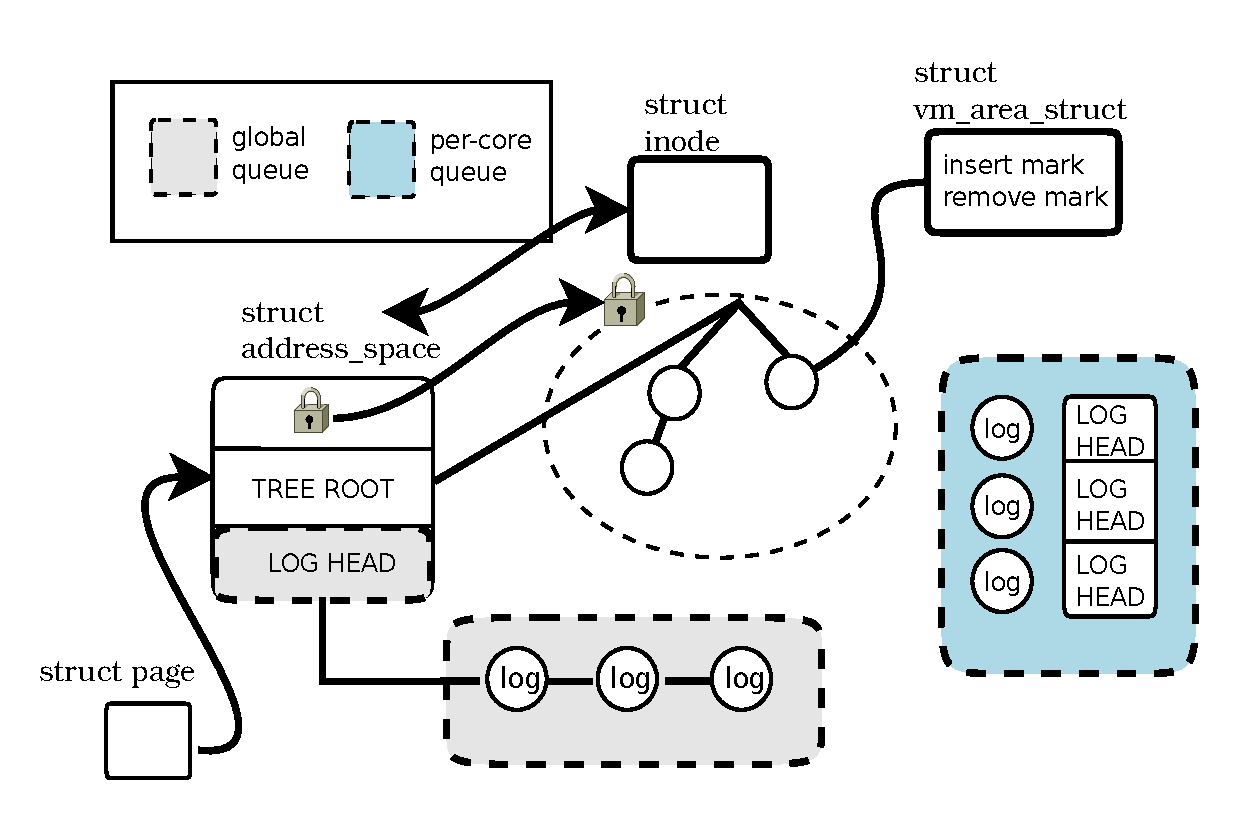
\includegraphics[width=1\textwidth,height=1\textheight,keepaspectratio]{fig/file_rmap}
  \end{center}
  \caption{An example of applying the \LDU to file reverse mapping. 
  The file rmap can be serialized at updating VMAs into the interval tree.
  The log's queue is added into the per-core memory or the
  global head object(\code{struct address\_space})}
  \label{fig:fileramp}
\end{figure}

%$$$$$$$$$$$$$$$$$$$$$$$$$$$$$$$$$$$$$$$$$$$$$$$$$$$$$$$$$$$$$$$$$$$$$$$$$$$$$$$$
%Paragraph 1: linux의 file mapped page reverse mapping의 구조에 대한 설명
%$$$$$$$$$$$$$$$$$$$$$$$$$$$$$$$$$$$$$$$$$$$$$$$$$$$$$$$$$$$$$$$$$$$$$$$$$$$$$$$$
Figure \ref{fig:fileramp} shows the rmap for file.
In order to translate physical addresses to virtual address, the page(\code{struct page})
indicates the address space object(\code{struct address\_space}), and
the address space object manages the VMAs by using the
interval tree.
This interval tree is a shared resource between processes.
%, so Linux kernel uses the reader-writer semaphore to protect the tree.
Because the system calls such as \code{fork()}, \code{exit()} and
\code{mmap()} entail concurrent updating VMAs into the shared resource.
when the processes simultaneously invoke these system calls, the
file rmap can be serialized at the update operations.

%$$$$$$$$$$$$$$$$$$$$$$$$$$$$$$$$$$$$$$$$$$$$$$$$$$$$$$$$$$$$$$$$$$$$$$$$$$$$$$$$
%Paragraph 2: file mapping에 ldu 적용한 방법에 대한 설명 
%$$$$$$$$$$$$$$$$$$$$$$$$$$$$$$$$$$$$$$$$$$$$$$$$$$$$$$$$$$$$$$$$$$$$$$$$$$$$$$$$
The \LDU can easily be applied to the file ramp data structure.
For instance, to use the \LDU, a developer adds log's queue header into the per-core
memory or into the original data structure(\code{struct address\_space}), and
then adds mark field to the individual object(\code{struct vm\_area\_struct}).
Then, the developer modifies update function to logging function without a lock.
Finally, the developer creates \code{synchronize} function and calls
the \code{synchronize} function before the read.
%the mark field adds to the individual object(\code{struct
%vm\_area\_struct}), and then the log's queue is added into the per-core
%memory or the global head object(\code{struct address\_space}).

This figure clearly shows why the \LDU additionally supports the
global queue because it is a simpler and easier scheme because the log's head
pointer is located in the interval tree's data structure.
On the other hand, the
per-core queue may need an additional per-core queue management scheme due
to the its isolated memory location.

\subsection{Detail Implementation}
%$$$$$$$$$$$$$$$$$$$$$$$$$$$$$$$$$$$$$$$$$$$$$$$$$$$$$$$$$$$$$$$$$$$$$$$$$$$$$$$$
%Paragraph 2: per-core queue 구현에 대한 설명 
%$$$$$$$$$$$$$$$$$$$$$$$$$$$$$$$$$$$$$$$$$$$$$$$$$$$$$$$$$$$$$$$$$$$$$$$$$$$$$$$$
Because the log's head pointer for the per-core queue is
separated with the original data structure, the implementation of
per-core queue uses 
a per-core hash table method that can allow each object to distinguish.
The per-core hash table implemented as a direct-mapped cache, which one
bucket only has an object because recently used objects will be in the hash
table in a way similar to the OpLog's per-core hash table.
When this hash table is met a hash conflict, the \LDU evicts the object in the
hash slot.
Moreover, this method reduces additional tasks of programmers because it can
minimize code modifications and does not need an additional lock.
The per-core hash table, however, incurs a hash conflict overhead.
This method is useful when a number of the root objects are infrequently created like the 
file rmap(\code{struct address\_space}).
On the other hand, since the anonymous rmap severely creates many
root objects(\code{struct anon\_vma}), it causes a hash conflict overhead.
Therefore, in the case of the anonymous ramp, we did not distinguish object
headers, but it needs additional tasks with global lock.

%$$$$$$$$$$$$$$$$$$$$$$$$$$$$$$$$$$$$$$$$$$$$$$$$$$$$$$$$$$$$$$$$$$$$$$$$$$$$$$$$
%Paragraph 1: 커널 버전 및 코드 분량, 테스트에 대한 설명
%$$$$$$$$$$$$$$$$$$$$$$$$$$$$$$$$$$$$$$$$$$$$$$$$$$$$$$$$$$$$$$$$$$$$$$$$$$$$$$$$
We have implemented the new deferred update algorithm in Linux 4.5-rc6 kernel,
and our modified Linux is available as open source. 
%The version of global queue modified code is xx that less complex, but per-core
%queue the modified code is xx-xx.
The implementation is stable enough and has passed the testing
related with virtual memory, scheduler,
and file in the Linux Test Project~\cite{LTP}.
